
\subsection{Densitat de malla}

La densitat de malla és el nombre de volums de control i de nodes en què discretitza espacialment el domini. Es diu que la malla és grollera si la discretització té pocs volums de control i es diu que la malla és fina si en té molts. Intuïtivament, una malla més fina donarà resultats més pròxims a la realitat.

Per l'anàlisi de la densitat de malla es pren una discretització uniforme, donada per la condició \eqref{eq:malla_uniforme}, i es fixa el valor de $N_1$, amb $N_1 \in \{ 5, \, 15, \, 25, \, 35, \, 45, \, 55\}$. L'esquema d'integració numèrica és Crank--Nicolson, amb $\Delta t = 1.00 \ \second$. Es calculen els mapes de temperatura en $t = 5000 \ \second$ i $t = 10000 \second$. La condició de convergència és novament $\delta = 10^{-11}$. 

En les representacions dels mapes de temperatura no s'interpola la temperatura dels nodes, sino que cada volum de control té assignada la temperatura del seu node. El motiu d'aquesta decisió es mostra a la figura \ref{fig:malla_comparacio}.
\begin{figure}[ht]
	\centering
	\begin{subfigure}{.5\textwidth}
		\centering
		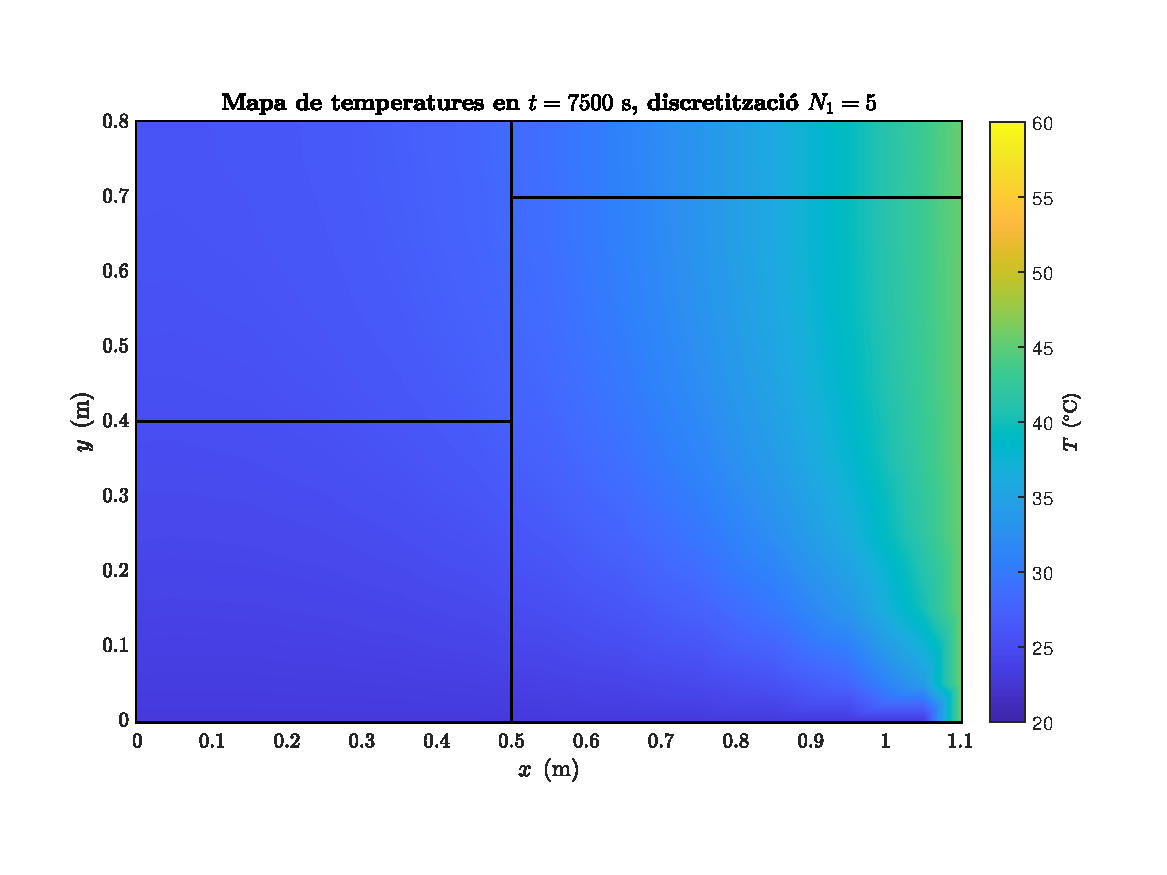
\includegraphics[width=.95\linewidth]{imagenes/04_influencia/malla/malla_31.pdf}
		\vspace{-15pt}
		\caption{Temps $t_\text{max} = 7500 \ \second$, discretització $N_1 = 5$.}
		\label{fig:malla_31}
	\end{subfigure}%
	\begin{subfigure}{.5\textwidth}
		\centering
		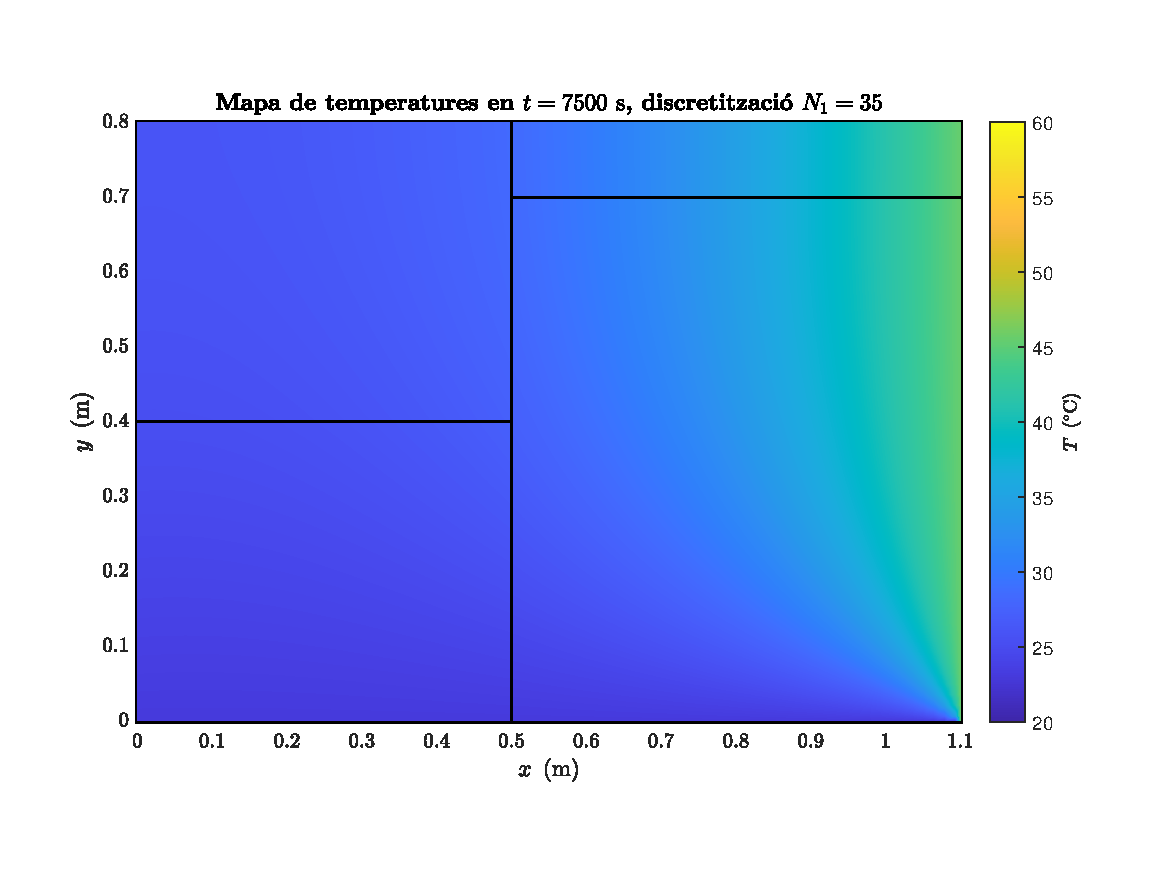
\includegraphics[width=.95\linewidth]{imagenes/04_influencia/malla/malla_34.pdf}
		\vspace{-15pt}
		\caption{Temps $t_\text{max} = 7500 \ \second$, discretització $N_1 = 35$.}
		\label{fig:malla_34}
	\end{subfigure}
	\caption{Mapes de temperatures en $t_\text{max} = 7500 \ \second$ i discretitzacions de $N_1 = 5$ i $35$ nodes, amb interpolació.}
	\label{fig:malla_comparacio}
\end{figure} 

\noindent
La discretització amb $N_1 = 35$ és molt més fina que amb $N_1 = 5$, de manera que dona millors resultats. Si s'interpola la temperatura entre nodes, aquesta diferència no s'aprecia.

Per a les diferents discretitzacions considerades, a les figures \ref{fig:malla_5000} i \ref{fig:malla_10000} es mostren els mapes de temperatures en $t = 5000 \ \second$ i $t = 10000 \ \second$, respectivament. En vista dels resultats obtinguts, es conclou que una discretització uniforme no és adequada. Dont que el gradient de temperatures en els materials $M1$ i $M3$ és petit, no és necessaria una discretització tan fina. En canvi, en la paret dreta el gradient de temperatures es major, requerint de major finura en la malla.

\begin{figure}[ht]
	\centering
	\begin{subfigure}{.5\textwidth}
		\centering
		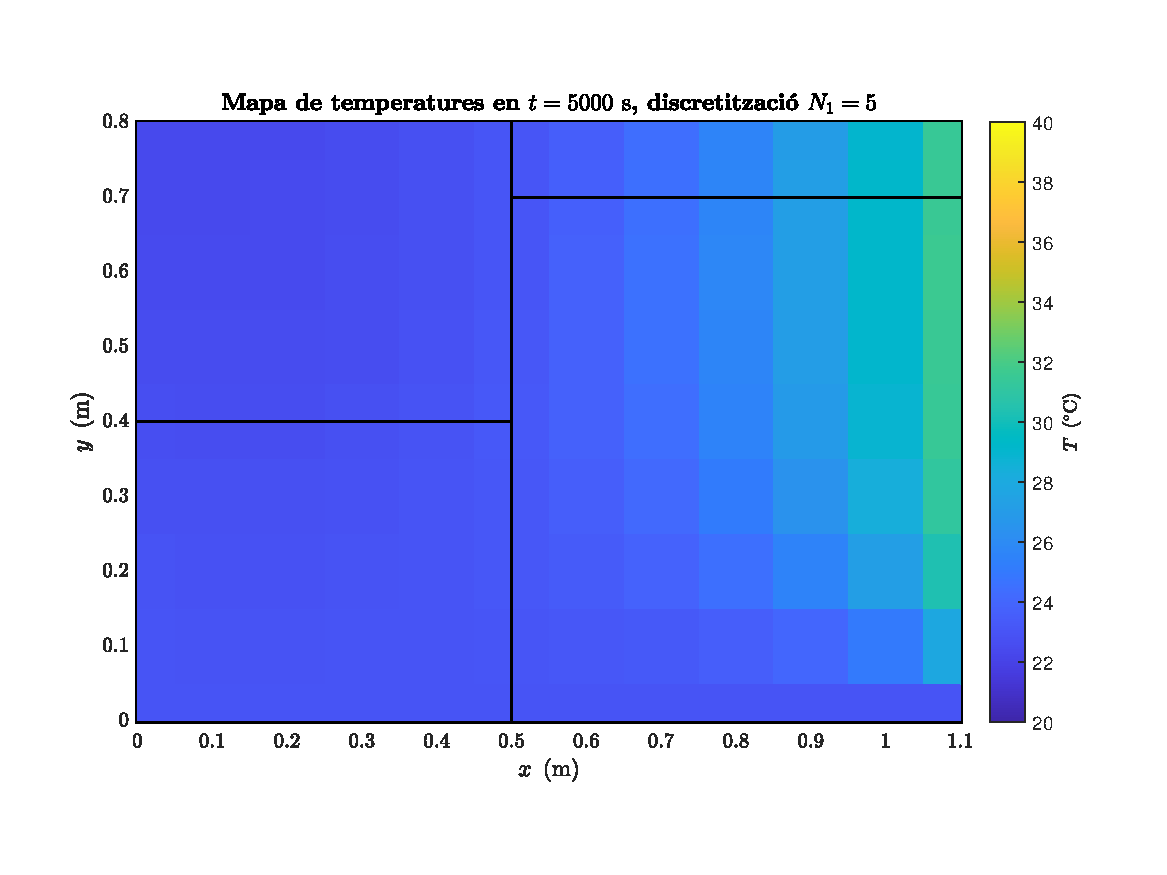
\includegraphics[width=.95\linewidth]{imagenes/04_influencia/malla/malla_1.pdf}
		\vspace{-15pt}
		\caption{Temps $t_\text{max} = 5000 \ \second$, discretització $N_1 = 5$.}
		\label{fig:malla_1}
	\end{subfigure}%
	\begin{subfigure}{.5\textwidth}
		\centering
		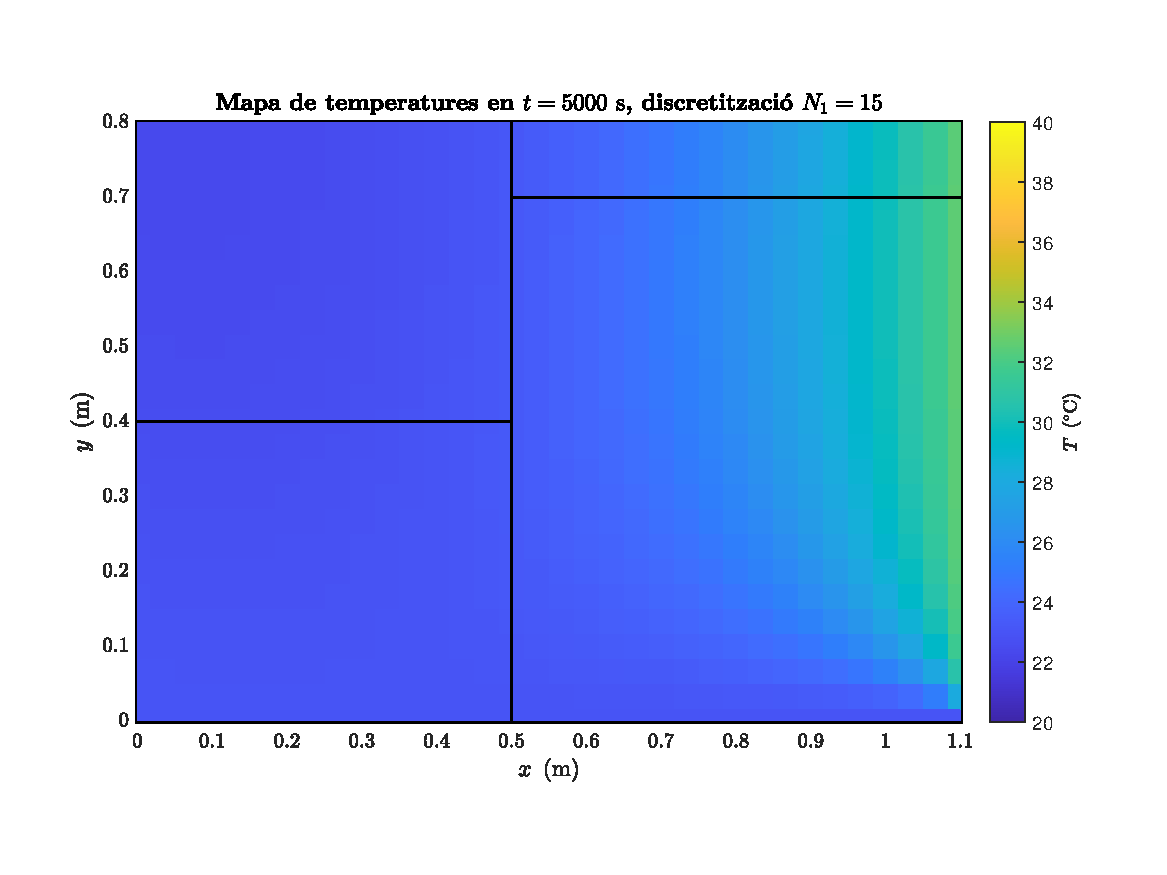
\includegraphics[width=.95\linewidth]{imagenes/04_influencia/malla/malla_2.pdf}
		\vspace{-15pt}
		\caption{Temps $t_\text{max} = 5000 \ \second$, discretització $N_1 = 15$.}
		\label{fig:malla_2}
	\end{subfigure}
	\begin{subfigure}{.5\textwidth}
		\centering
		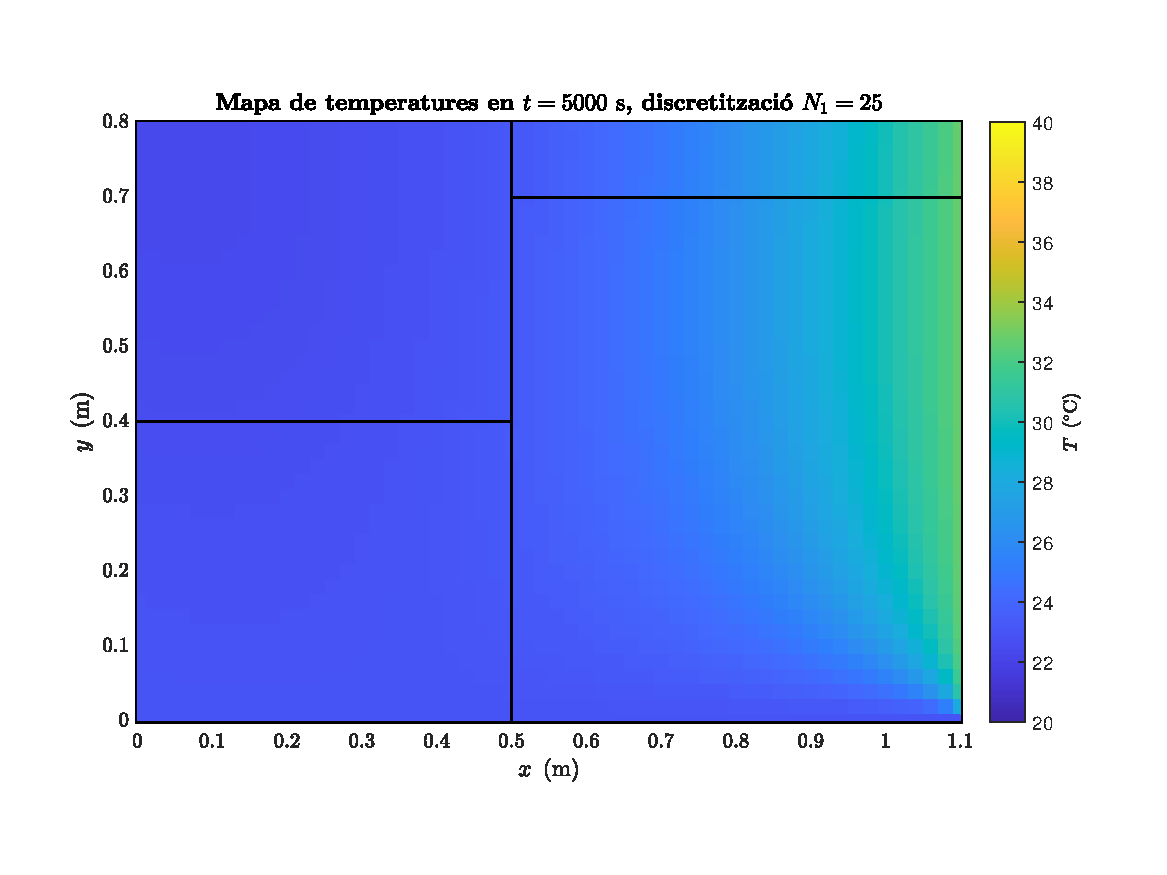
\includegraphics[width=.95\linewidth]{imagenes/04_influencia/malla/malla_3.pdf}
		\vspace{-15pt}
		\caption{Temps $t_\text{max} = 5000 \ \second$, discretització $N_1 = 25$.}
		\label{fig:malla_3}
	\end{subfigure}%
	\begin{subfigure}{.5\textwidth}
		\centering
		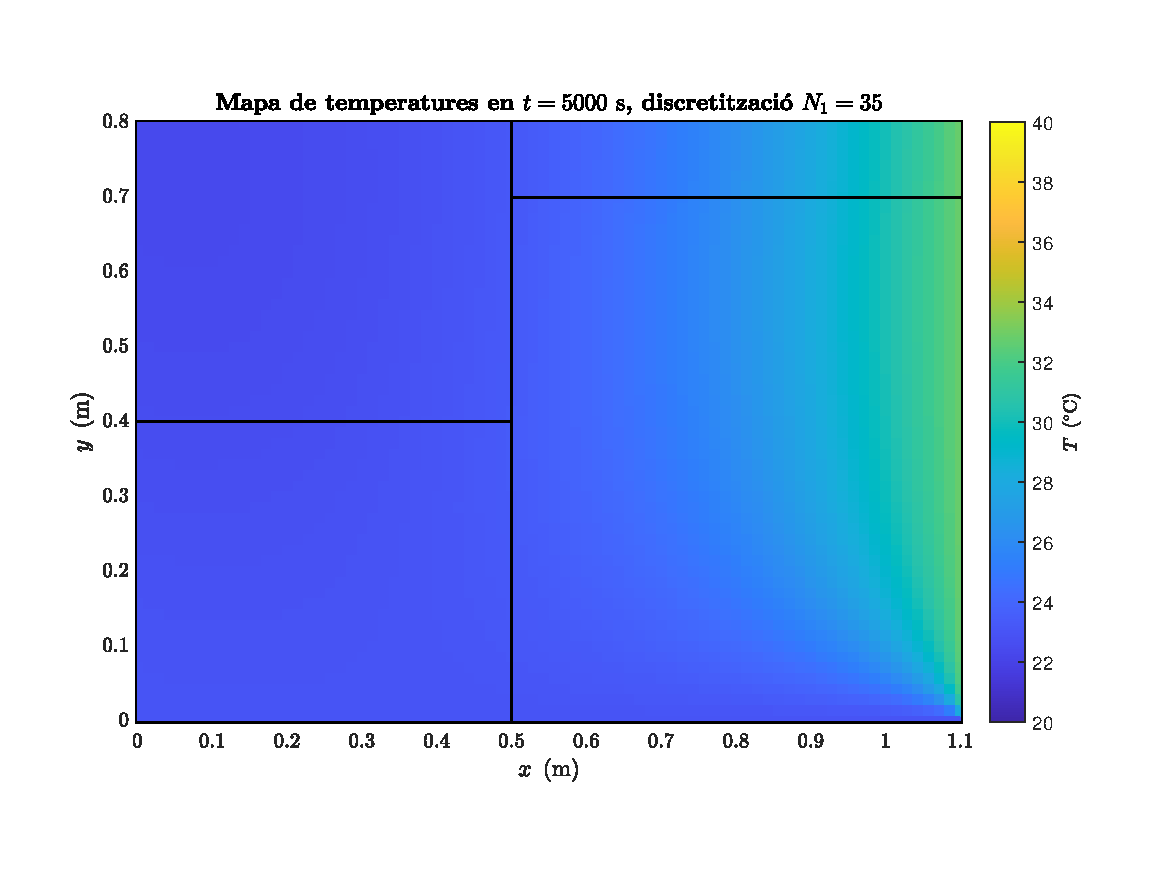
\includegraphics[width=.95\linewidth]{imagenes/04_influencia/malla/malla_4.pdf}
		\vspace{-15pt}
		\caption{Temps $t_\text{max} = 5000 \ \second$, discretització $N_1 = 35$.}
		\label{fig:malla_4}
	\end{subfigure}
	\begin{subfigure}{.5\textwidth}
		\centering
		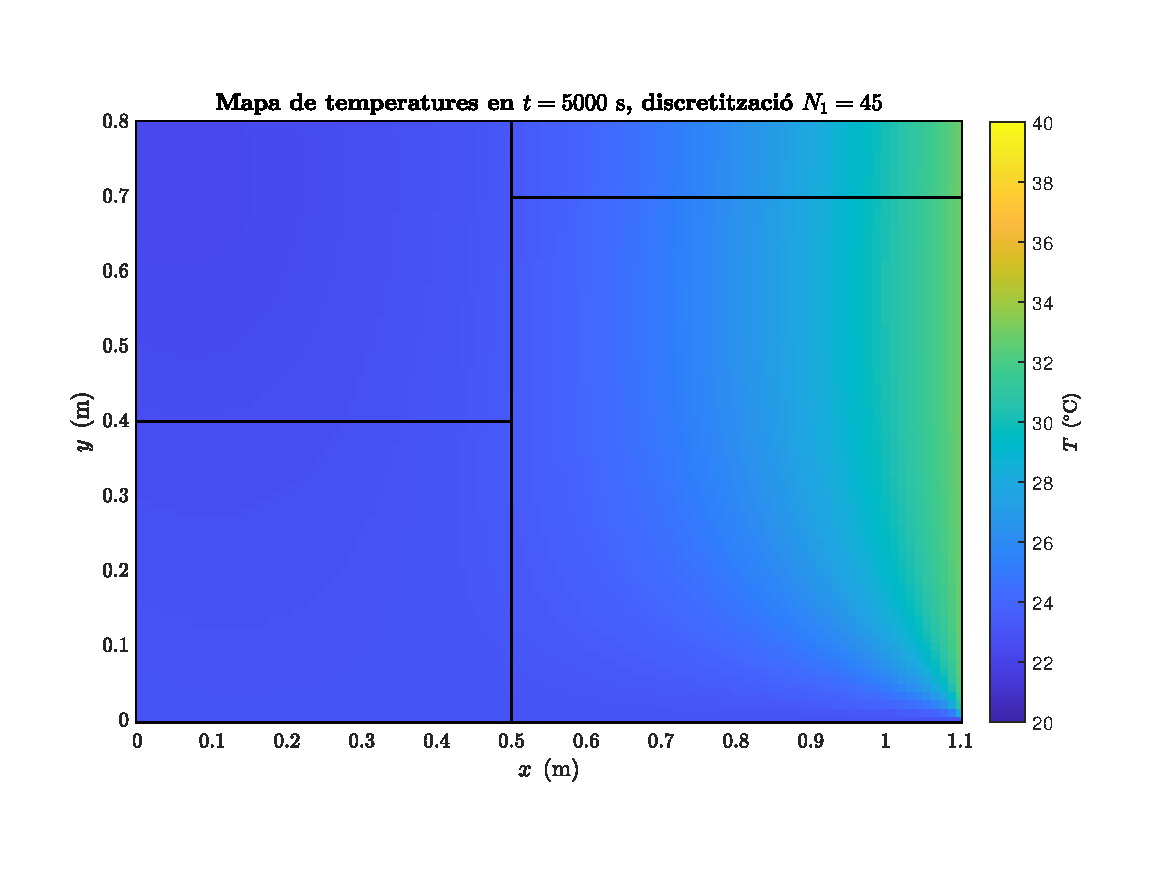
\includegraphics[width=.95\linewidth]{imagenes/04_influencia/malla/malla_5.pdf}
		\vspace{-15pt}
		\caption{Temps $t_\text{max} = 5000 \ \second$, discretització $N_1 = 45$.}
		\label{fig:malla_5}
	\end{subfigure}%
	\begin{subfigure}{.5\textwidth}
		\centering
		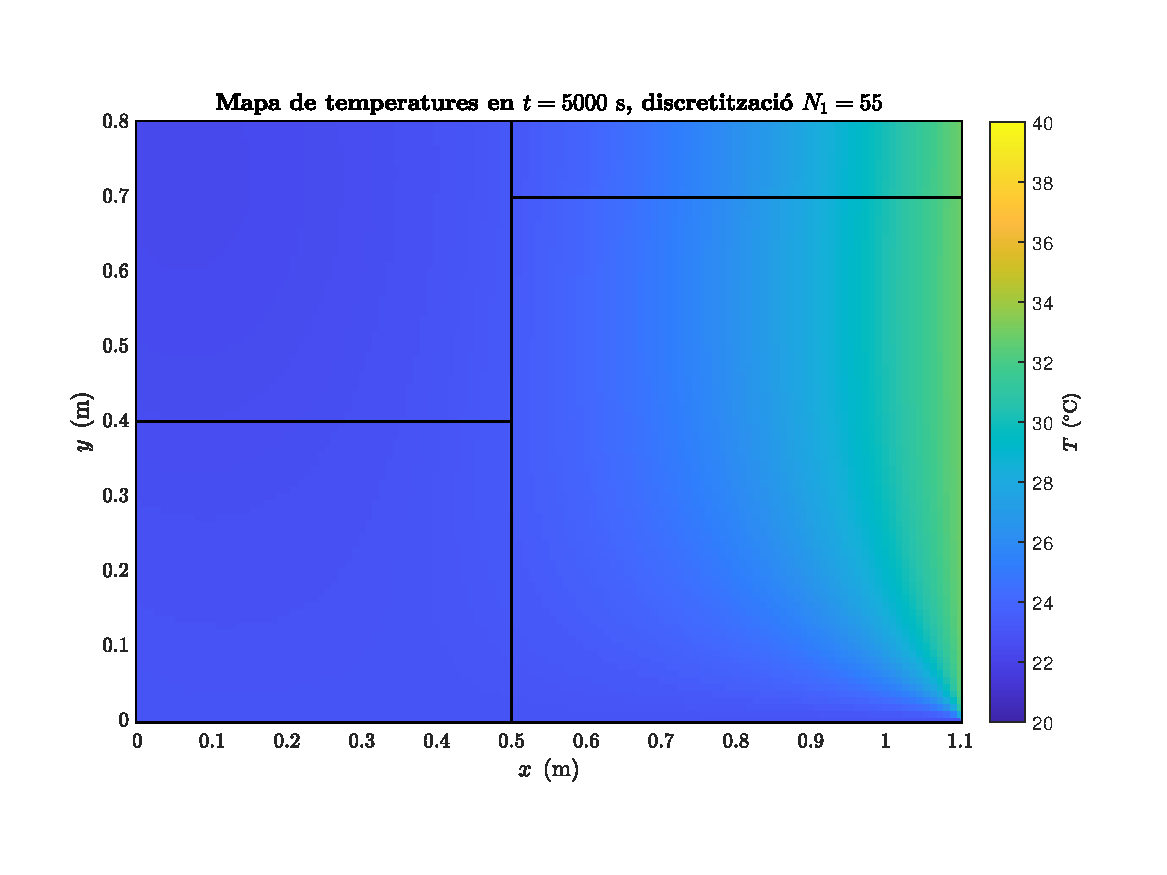
\includegraphics[width=.95\linewidth]{imagenes/04_influencia/malla/malla_6.pdf}
		\vspace{-15pt}
		\caption{Temps $t_\text{max} = 5000 \ \second$, discretització $N_1 = 55$.}
		\label{Temps fig:malla_6}
	\end{subfigure}
	\caption{Mapes de temperatures en $t_\text{max} = 5000 \ \second$, discretitzacions uniformes de $N_1 = 5, \, 15, \, 25, \, 35, \, 45$ i $55$ nodes, pas de temps $\Delta = 1.00 \ \second$, esquema Crank--Nicolson i sense interpolació. L'escala de temperatures és entre $20 \ \celsius$ i $40 \ \celsius$. Els materials amb temperatures més uniformes són $M1$ i $M3$. En aquests, la diferència entre discretitzacions espacials no és significativa. La zona amb un major gradient de temperatures és la paret dreta i la cantonada inferior dreta a causa de les condicions de contorn. En aquestes regions la millora en densificar la malla és notable. La discretització amb $N_1 = 45$ té $4582$ nodes, mentre que la discretització amb $N_1 = 55$ en té $7474$, la qual cosa incrementa el temps de càlcul. Com s'aprecia, la diferència entre ambdues discretitzacions en la regió amb major gradient tèrmic és petita.}
	\label{fig:malla_5000}
\end{figure} 

\begin{figure}[ht]
	\centering
	\begin{subfigure}{.5\textwidth}
		\centering
		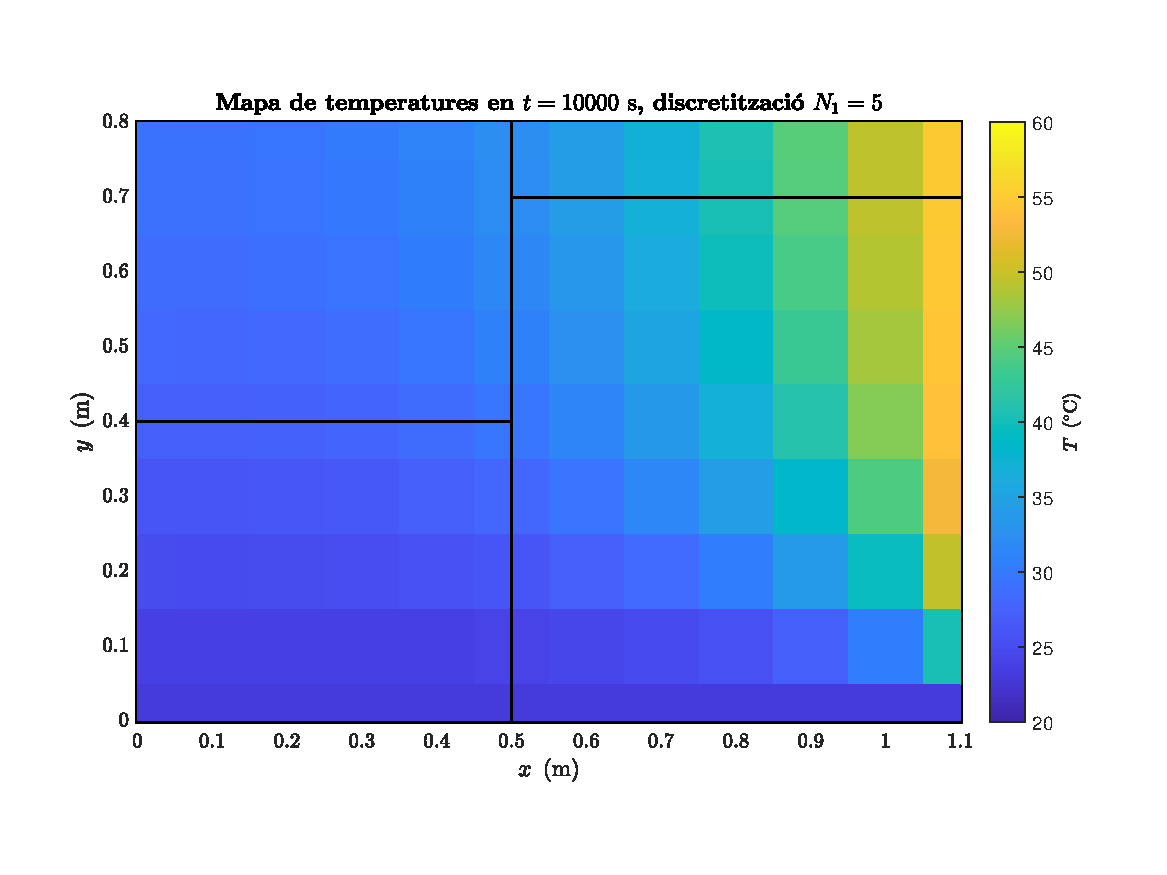
\includegraphics[width=.95\linewidth]{imagenes/04_influencia/malla/malla_7.pdf}
		\vspace{-15pt}
		\caption{Temps $t_\text{max} = 10000 \ \second$, discretització $N_1 = 5$.}
		\label{fig:malla_7}
	\end{subfigure}%
	\begin{subfigure}{.5\textwidth}
		\centering
		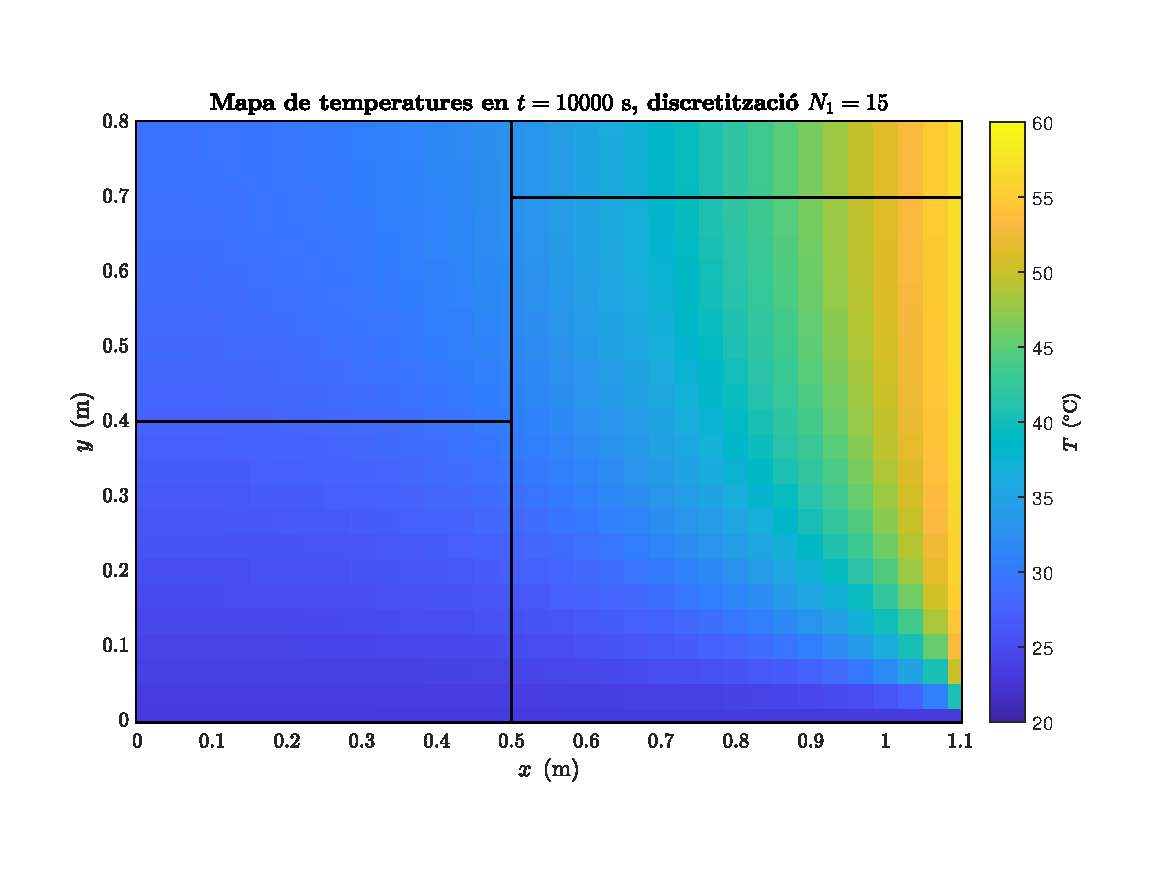
\includegraphics[width=.95\linewidth]{imagenes/04_influencia/malla/malla_8.pdf}
		\vspace{-15pt}
		\caption{Temps $t_\text{max} = 10000 \ \second$, discretització $N_1 = 15$.}
		\label{fig:malla_8}
	\end{subfigure}
	\begin{subfigure}{.5\textwidth}
		\centering
		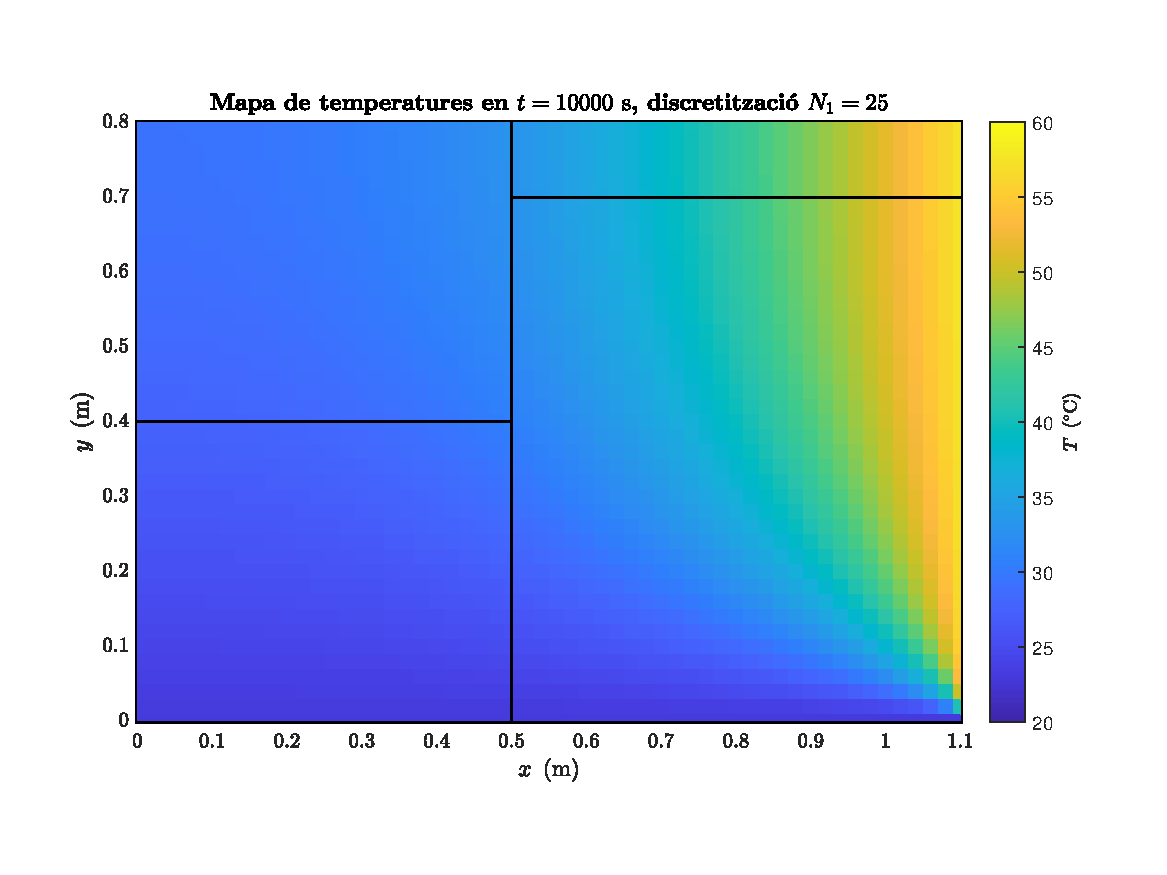
\includegraphics[width=.95\linewidth]{imagenes/04_influencia/malla/malla_9.pdf}
		\vspace{-15pt}
		\caption{Temps $t_\text{max} = 10000 \ \second$, discretització $N_1 = 25$.}
		\label{fig:malla_9}
	\end{subfigure}%
	\begin{subfigure}{.5\textwidth}
		\centering
		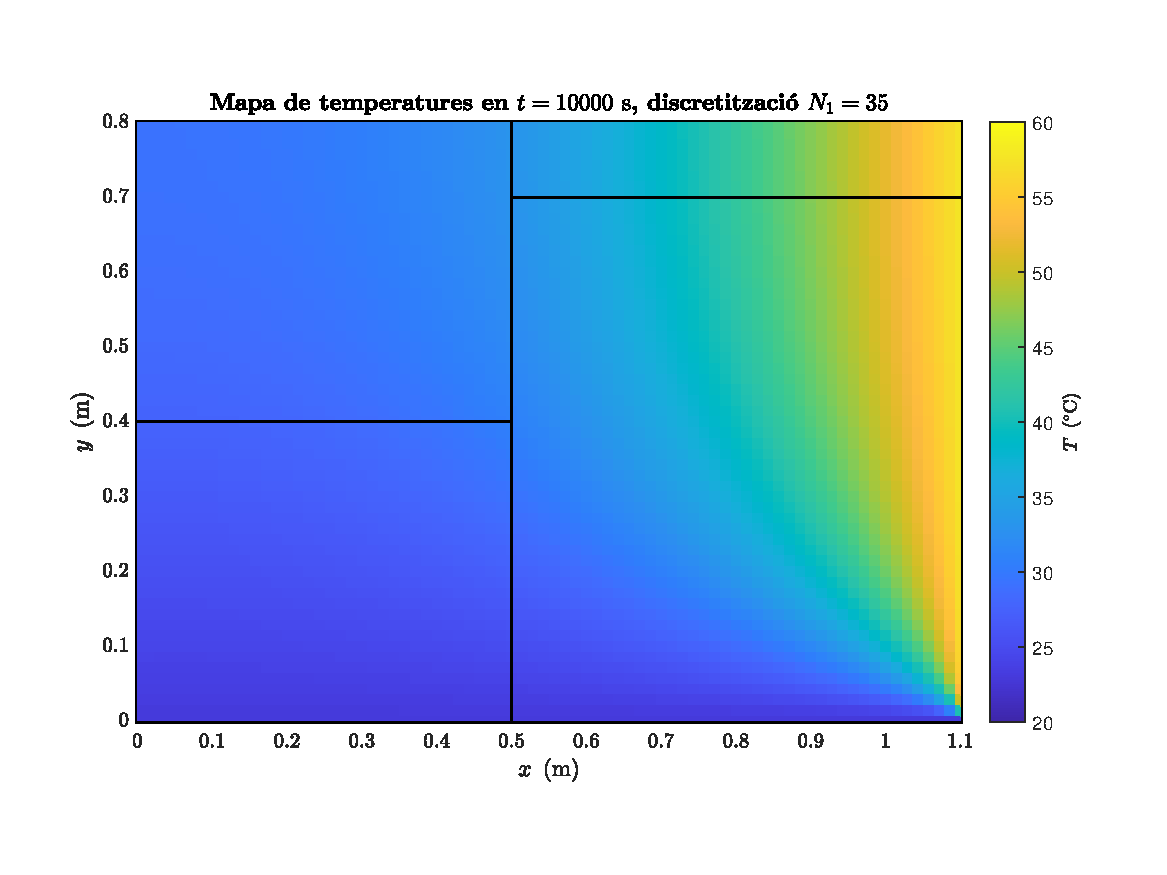
\includegraphics[width=.95\linewidth]{imagenes/04_influencia/malla/malla_10.pdf}
		\vspace{-15pt}
		\caption{Temps $t_\text{max} = 10000 \ \second$, discretització $N_1 = 35$.}
		\label{fig:malla_10}
	\end{subfigure}
	\begin{subfigure}{.5\textwidth}
		\centering
		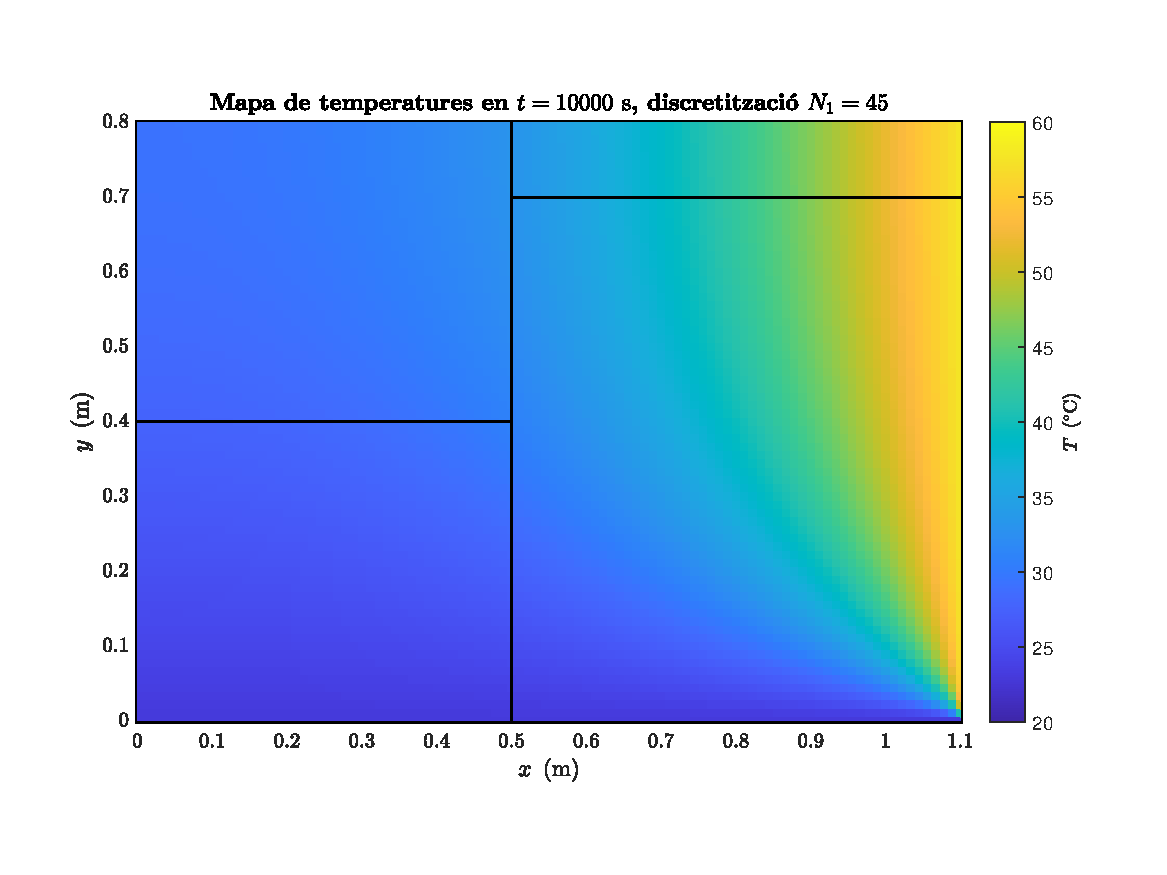
\includegraphics[width=.95\linewidth]{imagenes/04_influencia/malla/malla_11.pdf}
		\vspace{-15pt}
		\caption{Temps $t_\text{max} = 10000 \ \second$, discretització $N_1 = 45$.}
		\label{fig:malla_11}
	\end{subfigure}%
	\begin{subfigure}{.5\textwidth}
		\centering
		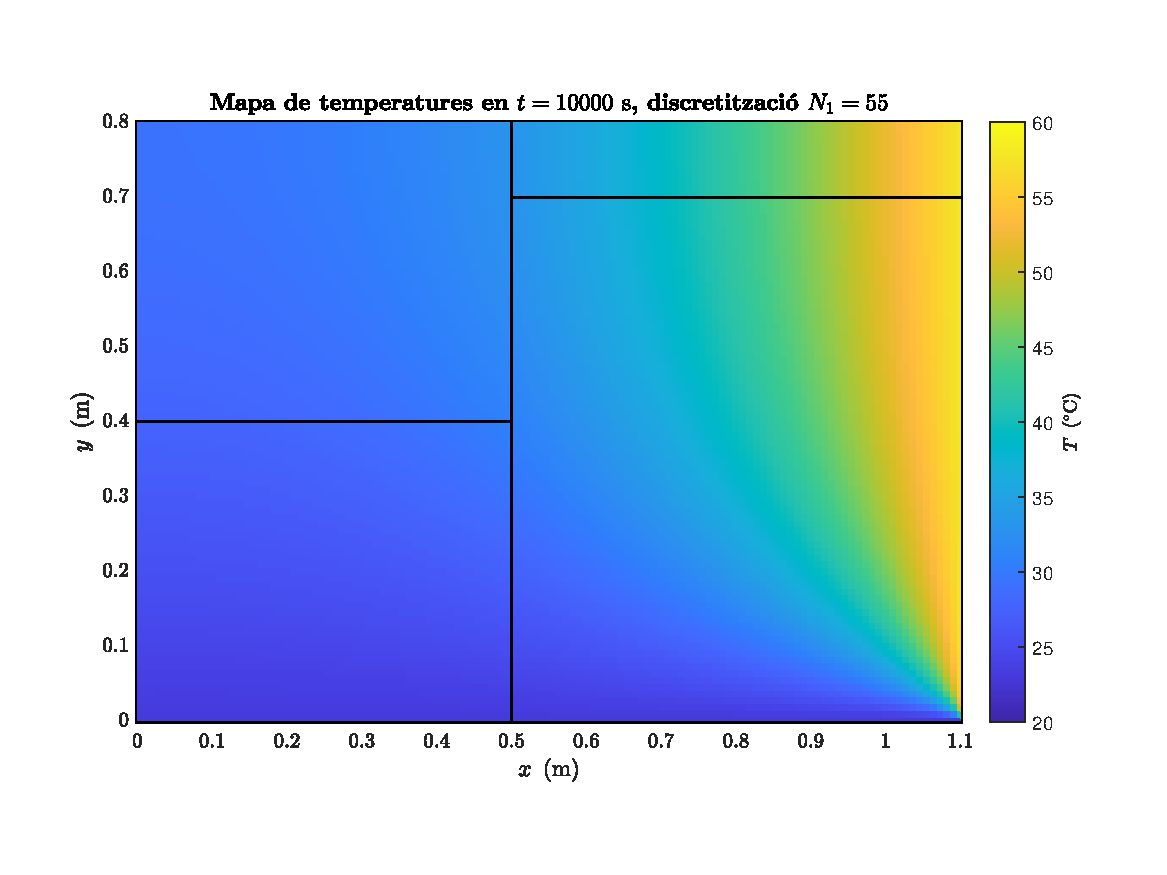
\includegraphics[width=.95\linewidth]{imagenes/04_influencia/malla/malla_12.pdf}
		\vspace{-15pt}
		\caption{Temps $t_\text{max} = 10000 \ \second$, discretització $N_1 = 55$.}
		\label{fig:malla_12}
	\end{subfigure}
	\caption{Mapes de temperatures en $t_\text{max} = 10000 \ \second$, discretitzacions uniformes de $N_1 = 5, \, 15, \, 25, \, 35, \, 45$ i $55$ nodes, pas de temps $\Delta = 1.00 \ \second$, esquema Crank--Nicolson i sense interpolació. L'escala de temperatures és entre $20 \ \celsius$ i $60 \ \celsius$. Els mateixos comentaris fets per $t_\text{max} = 5000 \ \second$ són aplicables al cas actual.}
	\label{fig:malla_10000}
\end{figure} 

\FloatBarrier